\documentclass{article}
\usepackage{amsmath}
\usepackage{graphicx}
\usepackage{float}
\usepackage{hyperref}
\usepackage{caption}
\usepackage{listings}

\title{CS 5720: Design and Analysis of Algorithms \\ Project 1 Report}
\author{Rachel Koch}
\date{\today}

\begin{document}

\maketitle

\section{Introduction}

The purpose of this project is to empirically analyze the time complexity of a brute-force search algorithm in terms of its worst-case, best-case, and average-case performance. The analysis is conducted using various sizes of character arrays derived from an English text and the algorithm is tested for different search characters (`e`, `m`, `Q`, and `\%`). We provide insights into the runtime of the algorithm and conjecture about the algorithm’s complexity based on the empirical results.

\section{Attributions}

ChatGPT file changes: \textit{second\_code.py}

\begin{quote}
\textbf{Overall Code Changes} \\
Changed the name of the file\\
Imported sys, numpy, and os packages, removed time \\
Reorganized code so it is in order of deliverable \\
Removed 'main' if-statement \\
Changed char array sizes because my text is shorter \\
Renamed the Search function and the arguments \\
Used a different book and url \\
Removed save$\_$text$\_$to$\_$file function, put code direct in body \\
Added logic to separate new best/worst/average dicts by char \\
Results are graphed differently based on character

\textbf{New Functions} \\
Added a newCharArray function to create arrays of random chars \\
Added a newChar function to generate a random character \\
Added a verificationTest function to test my search algorithm\\
Added wrapper for Python '$A[n]$.index' so it returns $n$ for 'not found' \\
Added a plot$\_$result function to plot only one case on one graph

\textbf{File Management} \\
VerificationTest, datasets, and experiment results get sent to a file \\
Added logic to remove results and dataset files if they exist already \\
Added success messages for data and graphs written to files

\textbf{download$\_$text() function} \\
Changed Start and End indices to match my book choice \\
Removed a line that only kept alphabetic and whitespace characters \\
Added code to remove carriage returns and newlines

\textbf{generate$\_$datasets() function} \\
Char array fill starts at beginning of text and pulls in chunks

\textbf{run$\_$experiments() function} \\
Changed time measurement to the index returned by Search()

\textbf{plot$\_$results() function} \\
Changed the y-axis label to just 'runtime', removed seconds

\end{quote}
ChatGPT file changes: \textit{second\_latex.tex}

\begin{quote}
Changed the name of the file\\
Added listings package \\
Added clearly delineated sections for deliverables \\
Section for Deliverable 1 shows algorithm and tests \\
Array sizes and book title changed in Deliverable 2 section \\
Added a reason for organizing results/graphs by character \\
Result graphs were all replaced \\
Result sections and conclusions were reorganized by character \\
Added an analysis of the results for each character
\end{quote}

\section{Deliverable 1: Search Algorithm}
\subsection{Algorithm}
\lstset{language=Python}
\begin{lstlisting}
def Search(A, K):
    for i in range(len(A)):
        if A[i] == K:
            return i
    return len(A)
\end{lstlisting}
A brute-force search algorithm that takes a character array \( A[n] \) and a search key \( K \). The algorithm returns the lowest index in \( A \) where \( K \) appears or \( n \) if \( K \) is not found.

\subsection{Verification}
Verification test results can be found in a file named \textit{test.txt}. Each test generated an array of random characters and compared the search results of both algorithms, indicating a pass/fail. Testing showed that the Search algorithm results and the Python list.index() function results matched in every case. A curated version of the results are shown below. \\ \\
\ttfamily
Verification Test \\
$[$'S', '*', 'u', '8', 'r'$]$ \\
Passed \\
K = 8 \\
Search =  3 \\
Index =  3 \\
\\
Verification Test \\
$[$ $]$ \\
Passed \\
K = r \\
Search =  0 \\
Index =  0 \\
 \\
Verification Test \\
$[$'P', 'J', 'w', 'l', 'z', 'Z', 'V', 'm', '?', 'Z', 'h', '!', 'A', 'e', 'b', 'h', 'x', '(', 'q'$]$ \\
Passed \\
K = ! \\
Search =  11 \\
Index =  11 \\
\\
Verification Test \\
$[$'q', 'F', 'V', '5', 'h'$]$ \\
Passed \\
K = X \\
Search =  5 \\
Index =  5 \\
\\
Verification Test \\
$[$'$\backslash$', 'n', 'y', 'g', '/', '6', '$\wedge$', '$\wedge$', 'j', 'T', 'g', '(', 'e', 'R', 'r', 'm', 'G', 'Y', 'n'$]$ \\
Passed \\
K = y \\
Search =  2 \\
Index =  2 \\
\\
\rmfamily
Additional test results are appended to the original \textit{test.txt} file every time the program is run.

\section{Deliverable 2: Dataset Generation}
To generate datasets for the empirical analysis, I used a public domain English text ("Folk Tales Every Child Should Know" by Hamilton Wright Mabie) downloaded from Project Gutenberg. The text was split into ten character arrays of varying lengths (100, 175, 250, ..., 775). For each array of length \( n \), 50 arrays were generated.

\section{Deliverables 3, 4, 5: Results}
Plots were split by character, and not by the worst/best/average case run-times, because it was easier to see and understand the patterns. For example, the best cases for characters 'e' and 'm' are so close that it was difficult to see their slight differences when graphed together. In another example, characters 'Q' and '\%' have the same worst/best/average cases. This led to the appearance of only one line when multiple were graphed together. In fact, the graphs for 'Q' and '\%' will be split into three graphs each (worst/best/average), so it can be clearly seen that all cases have the same run-time. The conclusion will include conjectures about the best, worst, and average case runtime of my algorithm.
	
\subsection{Character: \textit{e}}
Figure 1 shows the plot for best, worst, and average-case run-times of the test character 'e' in our Search algorithm.
    \begin{figure}[H]
	\centering
	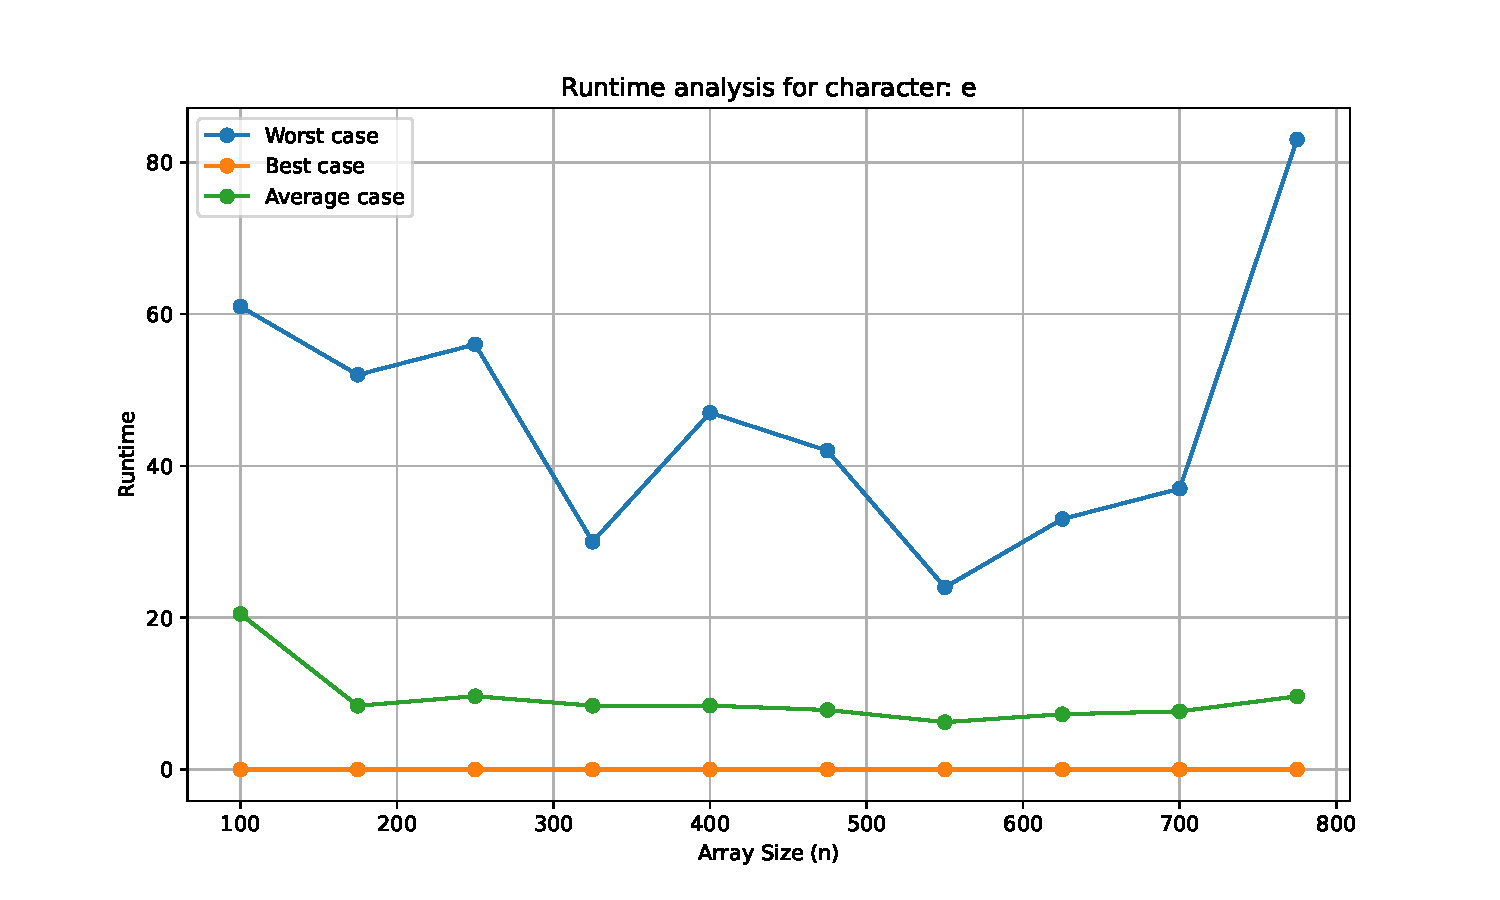
\includegraphics[width=\textwidth]{runtime_analysis_e.pdf}
	\caption{All run-times for character `e`.}
    \end{figure}

\begin{description}
    \item[Best-Case] As can be seen in Figure 1, the best-case runtime for 'e' was always zero. This means that there was always an array, in every set of length $n$, where 'e' was the first character in the array. This best case is $\Omega(1)$, so constant time.
    \item[Worst-Case] The worst-case line in Figure 1 never reaches the full length of the array, so this means that 'e' was found at least once in every array across all length $n$ arrays. This worst case is O$(n)$ because all the data points are some constant multiplied by array length $n$ ($\frac{n}{2}$, $\frac{n}{3}$, etc.).
    \item[Average-Case] The average case in Figure 1 is clearly between the best and worst cases, and skews towards the lower end. This is not surprising as 'e' is a very common character on English, and will almost always be found quickly (constant time) for large amounts of text. 
\end{description}


	
    \begin{itemize}
        \item Worst-case runtime: \( O(n) \)
	\item Best-case runtime: \( O(1) \)
	\item Average-case runtime: \( O(n) \)
    \end{itemize}
The results reinforce our understanding of brute-force search algorithms and their performance characteristics.

\end{document}